\begin{surferPage}[Yedigen]{Yedigen Simetrisine Sahip Bir Yedigil}
Yıldıza benzeyen bu yüzeyin derecesi  $7$.
Tekillik sayısı $84$; bu da yakın zamana kadar yedigiller üzerinde gerçel tekillik sayısı için bilinen en büyük sayıydı. Ta ki 2004'te  Oliver Labs dünya rekorunu $99$'a taşıyana kadar...
  
Etkileşimli görüntüde görülen üç yastık, Chmutov'un Sekizgilinde olduğu gibi, Çebişev polinomu kullanılmış olduğu için ortaya çıkmıştır.
Aslında yıldız şekilli bu yüzey Chmutov'un yüzeyinin bir çeşitlemesidir.
Burada $T_d(x)+T_d(y)$ ile verilen düzlem eğrisi, $S_7(x,y)$ ile göstereceğimiz bir düzgün yedigenle yer değiştirmiştir:
   \[S_7(x,y) + \lambda \cdot T_d(z) = 0.\]
Burada uygun bir $\lambda\in\RR$ değeri seçilmelidir. 
    \vspace*{-0.3em}
    \begin{center}
      \begin{tabular}{c@{\qquad}c}
        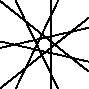
\includegraphics[height=1.5cm]{./../../common/images/labsseptic1.pdf}
        &
        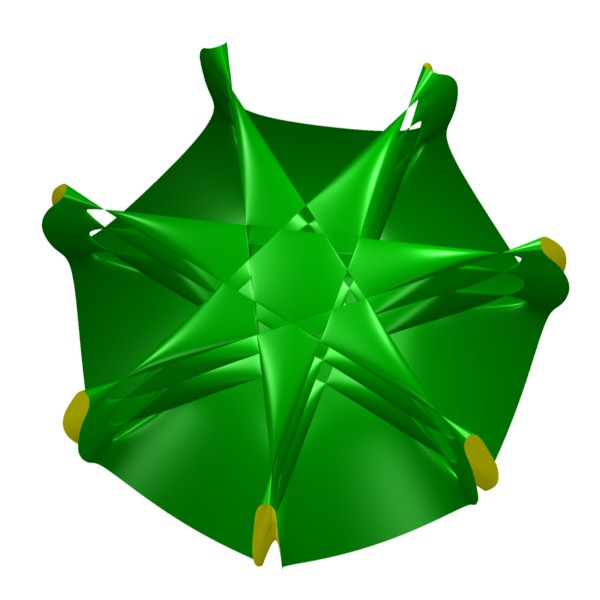
\includegraphics[height=1.5cm]{./../../common/images/septic_7eck_von_oben}
      \end{tabular}
    \end{center}
    \vspace*{-0.3em}   
Chmutov'un inşasının bu çeşitlemesi Duco van Straten tarafından verilmiştir.
\end{surferPage}
